\noindent The overall goals of the evaluation are:

\begin{enumerate}
  \item How can we provide a system that supports researchers interested in users participating in an energy competition?
	\item How can we effectively test the website and the overall design of the competition?
\end{enumerate}

% Since December of 2010, we held five user evaluations: one mockup evaluation, two onboarding evaluations, and two focus groups.

Since December of 2010, we held four user evaluations: one mockup evaluation, two onboarding evaluations, and a beta evaluation. We also have survey results from the inaugural Kukui Cup.

\section{Mockup Evaluation}
\label{eval-mockup}

\begin{figure}[h]
  \center
  \includegraphics[width=0.4\textwidth]{images/landing-mockup.eps}
  \caption{Mockup of the landing page.}
  \label{fig:landing-mockup}
\end{figure}

Before we stared implementing the beta version of Makahiki, we created mockups of the system in order to plan out what the new beta interface would look like. To create the mockups, we used a program called Balsamiq Mockups\cite{balsamiq-mockup}.  The mockups created by Balsamiq are visually simplistic by design; it conveys the idea that the mockups are not final and are subject to change.  At the same time, Balsamiq allows us to link together mockups, thus creating a mockup representation of the actual system's navigation. \autoref{fig:landing-mockup} is a mockup of the landing page, which is the first page users see when they visit the website.

After we finished creating our initial set of mockups, we held a user evaluation in December, 2010 of our ``mockup'' system.  The evaluation involved three scenarios.  The first scenario involved the user coming to the system for the first time, setting up their profile, making a commitment, and signing up for an event.  The second scenario was then having the user redeem a confirmation code for the event they said they would attend in the previous scenario and visit the ``Go Low'' page for the first time.  The final scenario involves viewing the list of prize winners and also seeing if they had earned any badges.

We invited colleagues, family, and friends to come in and go through the mockups.  When they came in, we gave them a brief overview of the competition (being careful to not provide too much information) and asked them to sign a consent form.  We then guided these subjects through the mockups instead of having them navigate through the system on their own.  While Balsamiq lets us link together mockups, it would be difficult to enumerate all possible paths through the mockups.  This is especially difficult because the state of many pages change after the user has done something (like participate in an event, for example).  Instead, in situations where there are several places that the user could go, we asked the user where they would like to go.  While the user may not always go where we want them to go, the hope is that most users will follow our scenarios.

During the evaluation, we asked the users to use a ``think out loud'' protocol.  We asked them to tell us what they are thinking, what they see, and what they want to do.  By doing this, we obtained additional insight into situations where users might get stuck.  We recorded both the audio and the computer screen of the guided tour using an application called ``ScreenFlow''.  As part of the consent form, we let the users know that their voice was being recorded and that only people working on the project will have access to this data. 

\section{Onboarding Evaluations}
\label{eval-onboarding}

After we finished the mockup evaluations, we started implementing the beta version of Makahiki using the mockups and user feedback.  We worked with a graphic designer at Windward Designs, who helped us develop our graphical design for the 2011 Kukui Cup.  By April of 2011, we were ready to have our first onboarding evaluation.  After we received feedback from the April evaluation, we held a second onboarding evaluation in July of 2011.

% May move into a different section
We use the term \emph{onboarding} to refer to the process that beginning and novice users go through early on in the game.  During this phase, we need to show the user the rules of the game and how it works.  Users coming to the Makahiki system for the first time may not know exactly what they have to do during the competition and will have little intuition for what they can do with the interface.  Within the Makahiki system, we have to provide sufficient guidance for these users in order to get users familiar with the interface.
% end section note

Unlike the mockup evaluations, we did not create any scenarios for the user.  Instead, we relied on the content of the quests and activities to get users acquainted with the interface.  While traditional usability evaluations use scenarios to evaluate how people complete tasks, using the content of the system provided a way for us to ``playtest'' our game. We also want to see how people interact with the system when someone is not guiding them through. These evaluations evaluate our ability to make a game as much as it evaluates our system's usability. Also, since the quests and activities are types of ``transactions'', we can measure the user's ability to complete them.

Each user that attended the evaluation was compensated in cash.  However, we also wanted to emulate the competitive environment, albeit on a smaller, individual scale.  Thus, we provided additional incentives that were available to the user during the evaluation. First, we created dummy users and simulated their participation in the website. If a user was able to get to first place against these sample users (the highest dummy user had 60 points), they earned additional cash.  Also, if the user allocated a raffle ticket in the raffle game to a gift certificate, we gave them the gift certificate.  In the beginning of each evaluation, we informed the users that they could earn these additional incentives.  However, we did not tell them how or where they would be able to earn it. The incentives were displayed to the user as quests and they appeared as the user progressed in the game.

We also asked participants to use the ``think out loud'' protocol.  We informed them that while they can ask questions, we may not be able to answer right away.  This is because we want to observe the subject when they do not have someone guiding them through.  We provided little guidance to the subject once they started playing the game.  We kept our interactions with the subject to a minimum. We stopped them after the first login sequence to get their feedback on the process.  We also asked the subjects for feedback whenever they watched a video to provide some feedback to the administrators who created the content. We used ``ScreenFlow'' again to capture the subject's voice and onscreen actions.

When the subjects came in, we had them sit in front of a Macbook Pro equipped with the latest versions of Firefox, Safari, and Google Chrome.  We then provided the subject with the guidelines of the evaluation and informed them that we are recording their voice and on screen actions.  They were then asked to sign a consent form. After the consent form was signed, we provided a little context about the system and the possible additional incentives. We then let the subject interact with the system unassisted for 30-40 minutes.  After that period, we answered any questions that may have come up, asked a few post-test questions of our own, and gave the subjects their compensation.  The script we used for the procedure can be found in Appendix A. We also made sure to dump the database after each subject for analysis before resetting the system to a pre-evaluation state.

Because these subjects were interacting with the system, we needed to have at least two people at each evaluation; one to observe the subject as they navigate through the system and ask questions and one to act as an administrator.  The person playing the administrator does not interact with the subject during the evaluation.  Their task is simply to review the submissions for tasks in the smart grid and choose to either approve or deny the subject's submission.  Because we are simulating the game on a small scale, the administrator needed to provide realistic feedback and encourage the subject to keep trying.

After the individual's time with the system was up, we asked them a few questions about their experience. These questions were based on questions in Krug's Don't Make Me Think~\cite{krug-dmmt}. The questions were:

\begin{itemize}
    \item What did you think about the website?
    \item What did you think about the background? Was it too cartoony?
    \item Is this something you think you and your friends would participate in? Why?
    \item What issues did you have while using the site?
    \item What can we do to improve the site?
\end{itemize}

For both of these evaluations, we recruited current residents of the Hale Lehua residence hall here at the University of Hawaii at Manoa, which was one of the residence halls participating in the 2011 Kukui Cup.  This residence hall was chosen because at the time of the first evaluation, it was the only residence hall in which we could get near-real time energy usage.  Since the residence halls in the competition are for first year students, these first-year students in 2010 would not be able to participate in the upcoming 2011 competition.

Once we had the screen recordings and the database dumps, we analyzed them to get a sense of how usable our system is. First, we looked at how long it takes a subject to complete workflows. Examples of workflows include the first login sequence, completing an activity, or completing a quest. The only workflow that is required of every subject is the first login sequence, so some subjects completed tasks that others have not. We also examined at the raw numbers from the database, including the number of points, number of quests completed, and the number of actions completed. We compared the evaluations with each other to see if there was improvement between iterations of the system. Of course, since a new subject is interacting with the system, we also took note of potential usability issues that each of the subjects have encountered. 

% \section{Focus Groups}
% 
% After each onboarding evaluation, we organized a focus group for users to attend.  These focus groups are primarily intended to provide a place where subjects that completed the onboarding evaluation can discuss the content of the system and what would motivate them and their floor-mates to compete.  However, it is also an opportunity to discuss their experiences with the system.  The audio of these sessions were recorded.

\section{Beta Evaluation}

Before deploying the website in production, we held a closed beta evaluation. Unlike the in-lab evaluations, this was more of a field test where subjects interacted with the website on their own time. Instead of using subjects from the towers, we recruited friends, family, and local organizations. This posed an issue: the energy and power information used in the Go Low page is directly tied to the energy in the Hale Aloha towers. We got around this by basing the energy use of the floors in the competition on the activity of the individuals in the floor. The number of points, the amount of wall activity, and the number of quests completed all contributed to this mocked energy data. However, the daily energy goal game was functional and awarded points to individuals of the team if their mocked energy consumption fell below the goal.

The duration of this evaluation was 6 days. The competition was divided into two rounds, with round two being an ``overall'' round. We purchased a few prizes for the winners as well as a few prizes to put in the Raffle Game.

After the beta test ended, we sent out a survey to the participants. This was a short 5 question survey that was used to get feedback for the system and the 2011 Kukui Cup. The questions were:

\begin{itemize}
  \item What aspects did you like most about the Kukui Cup beta test?
  \item What did you like least about the Kukui Cup beta experience?
  \item What suggestions (big or small) do you have for improving the Kukui Cup for our October launch at UH?
  \item What did you find to be your primary motivators and de-motivators for participating in the beta test?
  \item Any other comments you'd like to share with us?
\end{itemize}

This is an important component of our evaluation. Aspects of the website involve the passage of time (rounds, commitments, events, submission approval process) or interacting with others (social bonus, tickets in the raffle game, news page). The energy competition is also less about individuals and more about the group or floor as a whole. This was also an opportunity to test our mobile implementation and get a sense of how difficult the administration of the system might be.

Once again, we looked at the database to gather metrics on the performance of the evaluation participants. While we did not have screen recordings, we used our logging system to estimate how much time subjects spent in the system. This served as an early test of our logging component, which was used heavily to gather metrics from our production deployment. We also sent out a short survey to all of the beta evaluation participants for them to provide feedback on their experience using the system.

\section{Production Deployment}

In October 2011, we held the inaugural ``Quest for the Kukui Cup'', a residence hall energy competition here at the University of Hawaii at Manoa. The competition involved 1000 first-year students and resident advisors residing in the Hale Aloha Towers. This competition served as the first public deployment of Makahiki. In addition to the logs generated by Makahiki and the web server, we added a survey in the form of an activity to the Smart Grid Game in the last round of the competition. This survey included a few questions about the subject's experience with the website and what they felt we could improve.

\section{Summary}

These various evaluations contributed to our evaluation goals in different ways. Each type of evaluation satisfies a subset of our goals we outlined at the beginning of this chapter. Together, they provided us with a complete look at how individuals in the actual competition might have interacted with our site.

First, our mockup evaluation gave us insight into our design interface and whether or not it was intuitive. The benefit of the mockup evaluation was that we did could evaluate our interface before writing a line of code. This was critical because we did not want to waste time creating an interface that would be thrown away later. The downside of the mockup evaluation was that individuals did not directly interact with the mockups. Thus, we could not evaluate how these subjects interacted with the components. In addition, the lack of incentives made it impossible to evaluate our game design. Finally, the contents of the system was not developed at the time of the mockup evaluation, so we could not gain any insight into the content of the system.

The onboarding evaluation also gave us insight into our interface, but we also observed subjects interacting with the user interface components directly. Subjects were also interacting with the content of the system, so we also gained useful feedback that was forwarded to the content creators for the system. We also ``gamified'' the evaluation by providing incentives to do well in the system. This provided subjects with additional incentive to do well in order to get the full value out of the evaluation, but the way they were awarded was not an accurate representation of how the incentives would be awarded in an actual competition. Thus, while we gained some insight into our ability to make a compelling game, we needed to run a competition with multiple subjects over a period of time to fully evaluate our game design.

The beta evaluation was a more accurate representation of how the competition would be. Having multiple subjects interact with the site and compete against each other allowed us to more accurately evaluate the design of the actual competition. We also had more individuals interact with content, meaning that we could get even more feedback on the content of the web site. However, since individuals were interacting with the web site away from our lab, we could not directly observe their interactions with the web site.

